%%%%%%%%%%%%%%%%%%%%%%%%%%%%%%%%%%%%%%%%%
% Peking Univ. Physical Review (cn)
%
% LaTeX Template
% Version 2.1
% Release 03/19/18
%
% Original author:
% Mathias Legrand (legrand.mathias@gmail.com)
%
%%%%%%%%%%%%%%%%%%%%%%%%%%%%%%%%%%%%%%%%%
%
%----------------------------------------------------------------------------------------
%	PACKAGES AND OTHER DOCUMENT CONFIGURATIONS
%----------------------------------------------------------------------------------------
%\RequirePackage{times}      % Loads the Times-Roman Fonts
%\RequirePackage{mathptmx}   % Loads the Times-Roman Math Fonts
\documentclass[10pt,a4paper,twocolumn]{PPRAcn} % Document font size

\usepackage[UTF8]{ctex}
\usepackage[english]{babel} % Specify a different language here - english by default
\usepackage{lipsum} % Required to insert dummy text. To be removed otherwise
\usepackage{bm,caption,textcomp,subfigure,float}
\usepackage{flushend}
%\usepackage[keeplastbox]{flushend}
\usepackage{geometry}
\newgeometry{top=28mm,bottom=25mm,left=20mm,right=25mm}
\newcommand{\upcite}[1]{\textsuperscript{\textsuperscript{\cite{#1}}}}

%----------------------------------------------------------------------------------------
%	COLUMNS
%----------------------------------------------------------------------------------------

\setlength{\columnsep}{7.0mm} % Distance between the two columns of text
\setlength{\fboxrule}{0.75pt} % Width of the border around the abstract
\setlength{\abovecaptionskip}{5pt}
\setlength{\belowcaptionskip}{0pt}

%----------------------------------------------------------------------------------------
%	COLORS
%----------------------------------------------------------------------------------------

\definecolor{color1}{RGB}{0,0,90} % Color of the article title and sections
\definecolor{color2}{RGB}{0,20,20} % Color of the boxes behind the abstract and headings

%----------------------------------------------------------------------------------------
%	HYPERLINKS
%----------------------------------------------------------------------------------------

\usepackage{hyperref} % Required for hyperlinks
\hypersetup{hidelinks,colorlinks,breaklinks=true,urlcolor=color2,citecolor=color1,linkcolor=color1,bookmarksopen=false,pdftitle={Title},pdfauthor={Author}}

%----------------------------------------------------------------------------------------
%	ARTICLE INFORMATION
%----------------------------------------------------------------------------------------

\newcommand{\keywordname}{Keywords} % Defines the keywords heading name
\captionsetup[figure]{name={图}}
\captionsetup[table]{name={表}}
\captionsetup{font={small}}
%\JournalInfo{Journal, Vol. XXI, No. 1, 1-5, 2013} % Journal information
%\Archive{Additional note} % Additional notes (e.g. copyright, DOI, review/research article)

\PaperTitle{基于KCCA算法的EEG和语音特征融合情绪识别} % Article title


\Authors{刘晴\textsuperscript{1}*} % Authors

\affiliation{\quad\textsuperscript{1}\textit{西北工业大学}\qquad*\textbf{通讯作者}: elbox@qq.com}

\Abstract{\phantom{田田}
情绪识别是智能人机交互的重要环节。传统方法主要采用单模态情感特征进行识别,情感识别率低。针对该问题,本文提出了一种核典型相关分析算法(KCCA)的多特征(multi-features)融合情感识别方法。在特征层面上,分别选取外在直观表达信号——语音信号和生理信号——脑电波进行特征提取,然后利用两种特征互补性,采用核典型相关分析算法(KCCA)将它们进行融合,降低特征向量的维数。 最后选择SVM模型对情感识别的训练集进行建模,并通过具体情感数据集进行仿真实验.实验结果表明,核相关分析算法有效的提高了情感识别的正确率。
}


\Keywords{\phantom{田田} 情感识别\quad 核典型相关分析算法\quad 特征融合\quad 脑电特征}

 %这是标题,作者和摘要(关键词)

%----------------------------------------------------------------------------------------

\begin{document}

\flushbottom % Makes all text pages the same height

\maketitle % Print the title and abstract box

%\tableofcontents % Print the contents section

\thispagestyle{empty} % Removes page numbering from the first page

%----------------------------------------------------------------------------------------
%	ARTICLE CONTENTS
%----------------------------------------------------------------------------------------

\section{引言}
随着智能技术的发展,传统的人机交互方法已经不能满足人们的需求,在人机交互方向,人们不只满足于机器人对人的语言进行识别,机器人是否具备情绪识别能力是推进智能人机交互的关键。为了实现机器人与人类的自主情感交互,我们需要机器人有更高的情绪识别能力。

情绪识别在智能人机交互、机器人领域是十分值得探究的前沿热点方向。目前,情绪识别研究多数基于人的面部表情、语音和生理信号来进行。本文基于语音和生理信号的进行情绪识别。语音是一种情绪的外在表现,能够直观地反应说话人的情绪,但是,由于语音可能会被人为地伪装,有时难以检测到说话人的真实情绪。并且,单从语音信号来进行情绪分类识别,难以相近语音特征对应情绪(比如生气和惊讶)的识别。EEG 是人的生理反应,可以更直接地反映人的情感状态。然而EEG 信号复杂度高且十分微弱,并且原始EEG信号噪声来源较多,比如机器的工频干扰、电磁干扰,当人进行呼吸、眨眼、说话、晃动时均会对EEG 信号产生干扰。如果只用EEG 信号进行情绪分类,则会忽视人的外在情绪表现,而且受设备限制,在有些实际应用场景中难以有效执行。基于这两方面考虑,本文同时应用语音和EEG 信号,利用两种信号的互补特性,以提高情绪识别准确率。

在特征融合方面,简单的将多种情感特征组合到一起,不但特征维数高,运算代价大,识别慢,并且含有很多无效信息,影响识别率。为此有些学者提出采用主成分分析等算法对特征进行融合和选择,使识别效率得到提升。但PCA是一种线性特征融合算法,无法描述特征之间的非线性关系。本文提出了采用核典型相关分析算法(KCCA) 进行多特征融合。核典型相关分析(KCCA)是相关分析(CCA)的非线性扩展,CCA是一种非线性特征的提取方法,用核方法来增强典型相关分析方法,不仅能剔除冗余信息,增强鉴别信息,还能解决特征的线性不可分问题,挖掘非线性因素,具有更好的特征提取与表征能力。

\section{相关概念及介绍}
\subsection{支持向量机(SVM)算法}
在飞机家族中。无人机与载人飞机相较而言,有着机动性强,重量轻,体积小,无人员直接在支持向量机(SVM)分析是一种流行的机器学习工具,常用于分类和回归。SVM是由Vapnik于1995年首次提出的一种新颖的非线性学习方法。SVM具备坚实的理论基础,较好地实现了结构风险最小化原则,这是神经网络等其他机器学习方法不具备的。它通过对凸二次规划问题进行求解, 在有限样本学习能力与模型复杂度之间寻求折中, 以获取最佳泛化性能。图1为SVM体系结构图 \ref{fig:SVM},其中x(i)为输入的自变量特征值,K为核函数,通过核函数将自变量x(i)映射到高维特征空间,在该特征空间进行线性回归[2],得到输出Y。
\begin{figure}[!htbp]
    \centering
    %trim option's parameter order: left bottom right top
    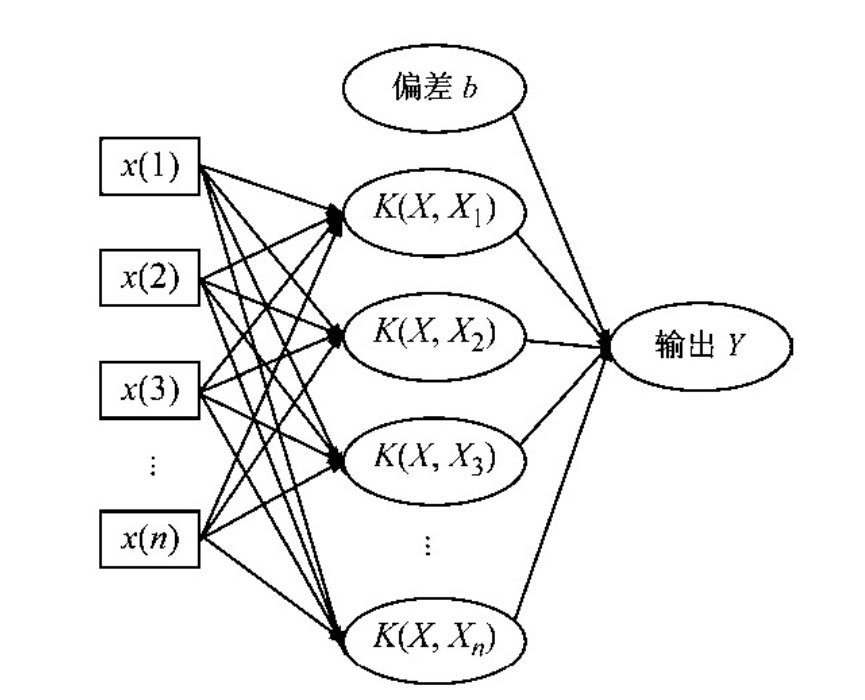
\includegraphics[width=7cm]{pic/svm.png}%trim = 0mm 0mm 0mm 0mm,clip,
    \caption{SVM体系结构。}
    \label{fig:SVM}
\end{figure}

当SVM用于处理回归问题时,目标是找到一个函数f(x),它对每个训练点x偏离$y_n$的值不大于ε,同时尽可能平坦。假设我们有一组训练样本,其中$x_n$是一个包含n个观测值的集合,$y_n$是对应的观测结果。
为了找到线性方程$f(x)=x′β+b$, 确保其足够平坦,需要找到满足最小范数$(β′β)$条件的f(x)。这是一个凸优化问题,以最小化$J(β)=12β′$β。

并满足如下等式:
\begin{equation}
\forall\ n:\left|y_n-\left(x_n^\prime\beta+b\right)\right|\le\varepsilon
\end{equation}

引入松弛变量后推出目标函数,也称为原始公式
\begin{equation}
J\left(\beta\right)=0.5\ast\beta^\prime\beta+C\sum_{n=1}^{N}{\xi_n+\xi_n^\ast}
\end{equation}

约束为:

\begin{equation}
\begin{gathered}
\forall\ n:y_n-\left(x_n^\prime\beta+b\right)\le\varepsilon+\xi_n\\
\forall\ n:\left(x_n^\prime\beta+b\right)-y_n\le\varepsilon+\xi_n^\ast\\
{\forall n:\xi}_n^\ast\geq0\\
\forall\ n:\ \xi_n\geq0
\end{gathered}
\end{equation}

常数C是框约束,是一个正数值,它控制对ε边界(ε)之外的观测值施加的惩罚,并有助于防止过度拟合(正则化)。该值决定了f(x)的平面度与允许大于ε的偏差量之间的权衡,用于寻求泛化性能与训练误差之间的折中。
线性ε-不敏感损失函数将观测值ε距离内的误差视为零而忽略。根据观测值y与ε边界之间的距离来测量误差。用如下的数学公式表示:

\begin{equation}
L_\varepsilon= 
\begin{cases}
0&               \text{if} |y-f(x)|\leq \varepsilon\\
|y-f(x)|-\varepsilon&       \text{otherwise}
\end{cases}
\end{equation}

\subsection{MVDR算法}
在介绍MVDR算法前,先引入相关线性滤波的知识[4]。
x是期望信号,为了得到x,需要对观测信号y进行线性滤波。

\begin{equation}
\begin{aligned}
z&=h^Hy\\
&= h^H\left(x+v_0\right)
&=x_{fd}+v_{rn}
\end{aligned}
\end{equation}

$v_0$是加性白噪声.z是x的估计,也是滤波器的输出信号,

\begin{equation}
h=\left[h_1h_2\ldots h_M\right]^T
\end{equation}

是长度为M的复数滤波器。

\begin{equation}
x_{fd}= h^Hx
\end{equation}

是期望滤波信号
\begin{equation}
v_{rn}=\ h^Hv_0
\end{equation}

是残差噪声。
\begin{equation}
I_M={Q'}_X{Q'}_X^H+{Q''}_X{Q''}_X^H
\end{equation}

${Q'}_X$是$M*R_X$维大小的矩阵,包含$\Phi_X$非零特征值对应的特征向量。
通过(9)可以把期望信号表示如下
\begin{equation}
\begin{aligned}
x&=Q_XQ_X^Hx
&={Q'}_X{Q'}_X^H\ x
\end{aligned}
\end{equation}

并从公式(10)推导出无失真约束
\begin{equation}
h^HQ_x'=i_i^TQ_x'
\end{equation}

\section{算法结合}
将公式(11)进一步推导为符合SVM目标函数的不等式约束
\begin{equation}
h^HQ_x^\le i_i^TQ_x'
\end{equation}

构造拉格朗日方程
\begin{equation}
\begin{aligned}
&J\left(w,\xi,{\xi^\prime}_i,a,a^\prime,\gamma,\gamma^\prime,\beta\right)=0.5||w||^2+C\sum\limits_{i=1}^{n}(\xi_i +\xi'_i)\\
&-\sum_{i=1}^{N}{a_i\left(w^Tx_i+b-d_i+\varepsilon+\xi_i\right)}\\
&-\sum_{i=1}^{N}{a_i\left(d_i-w^Tx_i-b+\varepsilon+{\xi'}_i\right)}\\
&-\sum_{i=1}^{N}{\beta_i\left(-h^HQ_{xi}'+i_i^TQ'\right)}
\end{aligned}
\end{equation}

\section{仿真实验}
为了测试该算法回归性能,在matlab上进行实验验证。设期望信号由五个谐波随机过程组成:$x\left(t\right)=\sum_{k=1}^{5}{A_kcos\left(2\pi f_kt+\phi_k\right)}$,其中振幅$A_k=0.5/k\left(k=1,\ldots,5\right)$,频率$f_k=0.05+0.1\left(k-1\right)\left(k=1,\ldots,5\right)$,随机相位$\phi_k$服从独立同分布,在区间0到$2\pi$上的均匀分布。需要在噪声观测下
$y\left(t\right)=x\left(t\right)+v\left(t\right)$恢复出原信号,v(t)是白噪声。SVM回归采用径向基函数( radial basis function,RBF),核函数中的参数$\gamma$和C的最优选取采用交叉验证自动选取,$\varepsilon$取0.00097。结果如图所示
\begin{figure}[!htbp]
    \centering
    %trim option's parameter order: left bottom right top
    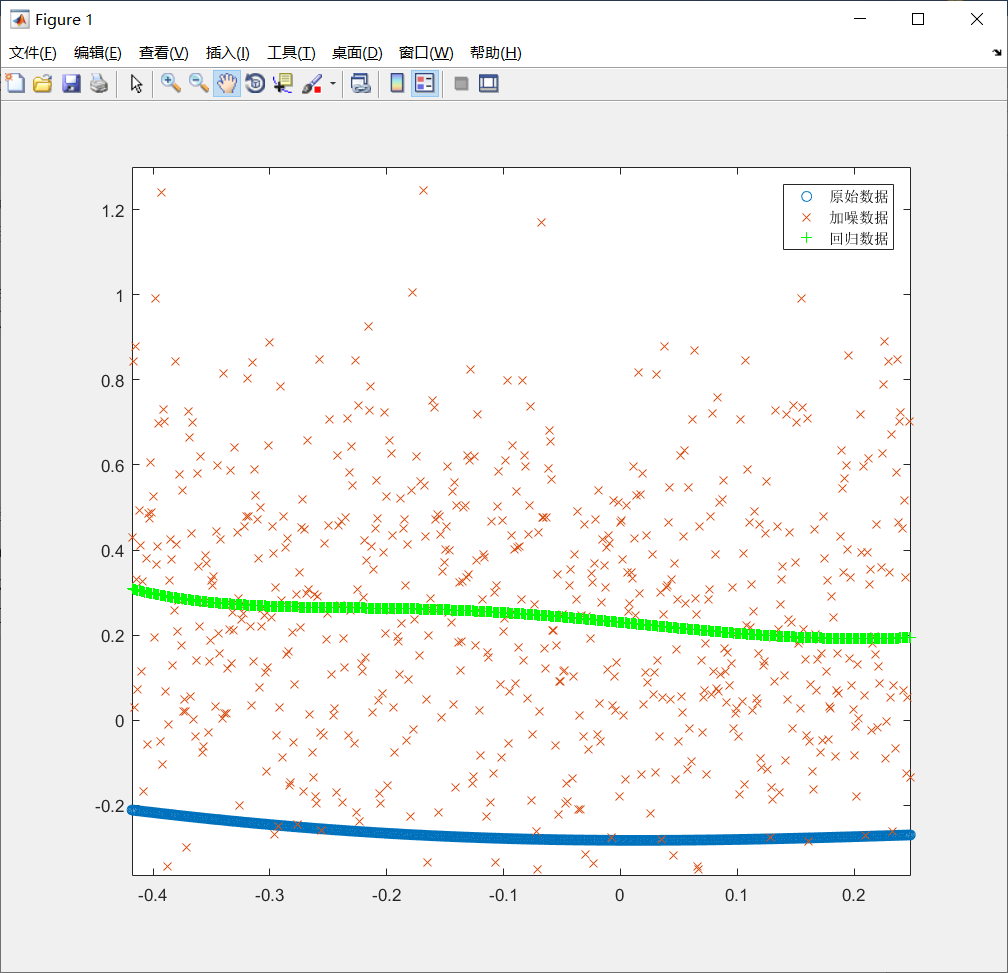
\includegraphics[width=7cm]{pic/res.png}%trim = 0mm 0mm 0mm 0mm,clip,
    \caption{处理结果。}
    \label{fig:res}
\end{figure}


\section{思考与改进}
总的来说本次仿真实验还有很多不足。首先在数据上由于相关知识的缺失,导致退而求其次并没有选择有色噪声而是选择了白噪声。由于MVDR的缺失导致最后在结果上也差强人意
 %这是正文

%----------------------------------------------------------------------------------------
%	REFERENCE LIST
%----------------------------------------------------------------------------------------

\phantomsection
\small
\renewcommand\refname{参考文献}
%\bibliographystyle{unsrt}
%\bibliography{essay/ref}

\begin{thebibliography}{99}
\bibitem{ref1}刘颖, 贺聪, 张清芳. 基于核相关分析算法的情感识别模型[J]. 吉林大学学报:理学版, 2017, 55(6):1539-1544.
\bibitem{ref2}刘付民, 张治斌, 沈记全. 核典型相关分析算法的多特征融合情感识别[J]. 计算机工程与应用, 2014, 50(9):193-196.
\bibitem{ref3}张前进, 王华东. 基于核典型相关分析和支持向量机的语音情感识别模型[J]. 南京理工大学学报, 2017, 41(2):191-197.  
\bibitem{ref4}林克正, 王海燕, 李骜,等. 高效求解方法的核典型相关分析算法[J]. 计算机科学与探索, 2017, 11(2):286-293.
\end{thebibliography}
%----------------------------------------------------------------------------------------

\end{document}
